\documentclass[11pt,a4paper]{article}

\usepackage{polski}
\usepackage[polish]{babel}
%\usepackage[none]{hyphenat} %no hyphen breaks
\usepackage[utf8]{inputenc}

%font
\usepackage[scaled]{helvet}
\renewcommand*\familydefault{\sfdefault}
\usepackage[T1]{fontenc}

\usepackage{color}

\usepackage{graphicx}

\usepackage{hyperref}

\usepackage{pdfpages}

\usepackage{tocloft}

%justify - no hyphens
\tolerance=1000
\emergencystretch=\maxdimen
\hyphenpenalty=1000
\hbadness=10000

%colors
\definecolor{darkyellow}{RGB}{244,213,9}
\definecolor{darkgreen}{RGB}{28,135,12}
\definecolor{darkishgreen}{RGB}{35,165,14}

\hypersetup{
    colorlinks,
    linkcolor=darkgreen,
    citecolor=blue,
    urlcolor=blue
}

\usepackage{fancyhdr}
\lhead{}
\rhead{}
\chead{\textsc{\textcolor{darkgreen}{PLQ Rulebook 2018-2020}}}
\cfoot{\thepage}
\renewcommand{\headrulewidth}{0pt}

\usepackage{enumitem}
%\setenumerate[1]{leftmargin=2.9cm,label=\Alph*.}
\setenumerate[1]{leftmargin=1.2cm,label=\textbf{\textcolor{darkgreen}{\Alph*.}}}
\setenumerate[2]{label=\textbf{\roman*.}}
\setenumerate[3]{label=\textbf{\alph*.}}
\setenumerate[4]{label=\textbf{\arabic*.}}

% Section numbering
\setcounter{secnumdepth}{5}
\setcounter{tocdepth}{2}

\usepackage{letltxmacro}

% Unnumbered sections included in ToC
\newcommand{\psection}[1]{
  \section*{#1}
  \addcontentsline{toc}{section}{#1}
}
\newcommand{\psubsection}[1]{
  \subsection*{#1}
  \addcontentsline{toc}{subsection}{#1}
}

\usepackage[explicit]{titlesec}
\usepackage{ulem}
\titleformat{\section}[block]{\center\normalfont\LARGE\bfseries}{\thesection.}{2ex}{#1}
\titleformat{\subsection}{\normalfont\Large\bfseries}{\textcolor{darkgreen}{\thesubsection.}}{1.5ex}{\textcolor{darkgreen}{\textsc{#1}}}
\titleformat{\subsubsection}{\normalfont\normalsize\bfseries}{\thesubsubsection.}{1ex}{#1}
\titleformat{\paragraph}[block]{\normalfont\normalsize}{}{0pt}{\uline{\theparagraph.\hspace*{1ex}#1}} %

%custom spacing
\newcommand{\sectionbreak}{\clearpage} %section starts on new page
% \titlespacing*{\subsection}{0.5cm}{0pt}{0pt}
\titlespacing*{\subsubsection}{0pt}{0.5cm}{-0.1cm}
%\titlespacing*{\paragraph}{2cm}{0pt}{0pt}

% Indent subsubsections
\newenvironment{indentpar}[1]%
  {\begin{list}{}%
          {\setlength{\leftmargin}{#1}}%
          \item[]%
  }
  {\end{list}}

\LetLtxMacro{\oldsubsection}{\subsection}
\renewcommand{\subsection}[1]{
  \oldsubsection{#1}%
  \label{\thesubsection}
}
\LetLtxMacro{\oldsubsubsection}{\subsubsection}
\renewcommand{\subsubsection}[1]{
  \oldsubsubsection{#1}%
  \label{\thesubsubsection}
}

\newcommand{\myref}[1]{\ref{#1}. \nameref{#1}}

\newlistof{bcc}{lbc}{\Large\textcolor{blue}{\textbf{Niebieska Kartka}}}
\newlistof{ycc}{lyc}{\Large\textcolor{darkyellow}{\textbf{Żółta Kartka}}}
\newlistof{rcc}{lrc}{\Large\textcolor{red}{\textbf{Czerwona Kartka}}}
\newlistof{pdc}{lpd}{\Large\textcolor{darkgreen}{\textbf{Pozostałe kary}}}

% Custom subparagraphs
\newcommand{\redcard}[1]{%
  \refstepcounter{rcc}
  \textcolor{darkgreen}{\textbf{Kara: }}\textcolor{red}{\textbf{Czerwona Kartka}} -- #1
  \addcontentsline{lrc}{rcc}{\numberline{\thesubsubsection} \hspace{3ex}#1}
}
\newcommand\yellowcard[1]{%
  \refstepcounter{ycc}
  \textcolor{darkgreen}{\textbf{Kara: }}\textcolor{darkyellow}{\textbf{Żółta Kartka}} -- #1
  \addcontentsline{lyc}{ycc}{\numberline{\thesubsubsection} \hspace{3ex}#1}
}
\newcommand\bluecard[1]{%
  \refstepcounter{bcc}
  \textcolor{darkgreen}{\textbf{Kara: }}\textcolor{blue}{\textbf{Niebieska Kartka}} -- #1
  \addcontentsline{lbc}{bcc}{\numberline{\thesubsubsection} \hspace{3ex}#1}
}
\newcommand\penaltyd[2]{%
  \refstepcounter{pdc}
  \textcolor{darkgreen}{\textbf{Kara: #1}} -- #2
  \addcontentsline{lpd}{pdc}{\numberline{\thesubsubsection} \hspace{3ex}#1 -- #2}
}

\usepackage{geometry}

\newcommand\image[2]{
	\newgeometry{left=0cm,top=#2}
	\includegraphics[width=\paperwidth]{#1}
	\restoregeometry
}

\setlength{\headheight}{13.6pt} %header

\setlength{\parindent}{0pt} % brak wcięć
\setlength{\parskip}{1ex plus 0.5ex minus 0.2ex}
\normalem %emphasis isn't underline
\linespread{1.1} %interlinia

\title{Zasady gry w~quidditcha}
\author{Polska Liga Quidditcha}
\date{Sezon 2018 - 2020}

\begin{document}

\maketitle
\clearpage

\setlength{\parskip}{0ex}

\pagestyle{fancy}

\tableofcontents

\setlength{\parskip}{1ex plus 0.5ex minus 0.2ex}

\newpage

\psection{Wstęp}

Popularność quidditcha stale rośnie i~rozwija się on w~dynamiczną i~ambitną dyscyplinę sportową,
wymagającą nie lada wysiłku fizycznego,
złożonych strategii i~nielichych umiejętności.

Każdego dnia treningi i mecze quidditcha odbywają się w 40 krajach na całym świecie.
W ciągu ostatnich dwóch lat ten sport przeżył niesamowity skok w rozwoju, co oznacza,
że zasady również muszą być rozwijane. Bazując na opiniach graczy, sędziów i trenerów
dokonaliśmy odpowiednich modyfikacji, mających polepszyć przyszłość quidditcha.

Rulebook został skondensowany, część zasad lepiej wyjaśniona, a niektóre elementy gry
zmienione. Mamy nadzieję, że te zmiany pomogą ustalić poprawny kierunek dla sportu, aby gracze
z całego świata byli podekscytowani quidditchem.

To wydanie \emph{Zasad gry w~quidditcha} opiera się na Rulebooku 2018-2020 wydanym przez IQA.

Polska Liga Quidditcha dziękuje wszystkim zaangażowanym (w kolejności alfabetycznej) w stworzenie przekładu niniejszych \emph{Zasad} z języka angielskiego:
\begin{center}
	\begin{tabular}{c c}
    Marian Dziubiak & Paulina Hausner \\
    Barbara Kulesza-Gulczyńska & Monika Maćkowiak \\
	\end{tabular}
\end{center}

%\image{team_poland}{6cm}
\pagebreak

% TODO: load from markdown

\newpage

\psection{DODATEK A: Definicje}
\leftskip0cm

\textbf{Bezbronny łapacz} -- Zawodnik, który jest w trakcie łapania piłki lecącej w powietrzu. Nie musi opuścić ziemi, żeby być bezbronnym. Nielegalne jest popychanie, szarżowanie, obejmowanie lub przewracanie bezbronnego łapacza (patrz \myref{6.1.7}).

\textbf{Celowy} -- Akcja wykonana świadomie i z zamierzeniem.

\textbf{Chroniony obrońca} -- Patrz \myref{7.2.2}.

\textbf{Czas gry} -- Oficjalny czas każdej gry, mierzony od pierwszego ,,M'' w ,,Miotły w górę'' do końca etapu gry, ale zatrzymywany na czas wstrzymań gry i pomiędzy etapami gry.

\textbf{Czas kary} -- Czas jaki zawodnik musi spędzić w strefie kar po popełnieniu faulu. Czas kary jest mierzony w czasie gry, więc nie płynie podczas przerw w grze.

\textbf{Dobry gol} -- Drużyna zdobywa 10 punktów gdy, po przełożeniu kafla w całości przez dowolną z pętli przeciwnika, sędzia potwierdzi gol (patrz \myref{4.1.1}).

\textbf{Dogrywka} -- Dodatkowy etap gry, następujący jeśli złapanie znicza w podstawowym czasie gry skutukowało remisem. Dogrywka trwa 5 minut czasu gry lub do złapania znicza (patrz \myref{3.5.3}).

\textbf{Druga dogrywka} -- Dodatkowy etap gry następujący jeśli dogrywka zakończyła się remisem. Druga dogrywka trwa dopóki jedna z drużyn nie strzeli bramki lub złapie znicza (patrz \myref{3.5.4}).

\textbf{Etap gry} -- Jeden z trzech możliwych etapów gry. Podstawowy czas gry trwa minimum 18 minut i do złapania znicza. Jeśli złapanie znicza skutkuje remisem, to odbywa się dogrywka. Jeśli po zakończeniu dogrywki nadal jest remis, to odbywa się druga dogrywka do pierwszego punktu.

\textbf{Gra} -- Pojedyncze starcie dwóch drużyn w celu określenia zwyciężcy.

\textbf{Granica boiska} -- Prostokąt 33 na 60 metrów ograniczający pole do gry (patrz \myref{2.1.1}).

\textbf{Immunitet} -- Zawodnik posiadający immunitet nie zostaje zbity po uderzeniu przez żywy tłuczek. Chroniony obrońca ma immunitet w swoim polu obrońcy. Pałkarz idący po trzeci tłuczek może zgłosić immuntet podnosząc rękę (patrz \myref{5.5.2}).

\textbf{Kafel} -- Piłka używana przez ścigających i obrońców do strzelania bramek (patrz \myref{2.3.1}).

\textbf{Kopnąć} -- Uderzyć stopą lub inną częścią nogi poniżej kolana. W momencie kopnięcia, zawodnik uderzający piłkę jest w jej posiadaniu jeśli jest jedyną osobą jej dotykającą. Każdy zawodnik może kopnąć piłkę raz, zanim zostanie ona podniesiona. Nielegalne jest kopanie przeciwnika.

\textbf{Lekkomyślna} -- Gra bez przemyślenia skutków swoich akcji.

\textbf{Martwy kafel} -- Kafel w czasie po strzeleniu bramki, przed rozpoczęciem gry przez obrońcę (patrz \myref{4.2.1}).

\textbf{Martwy tłuczek} -- Tłuczek, który nie powoduje zbicia (patrz \myref{5.2.2}).

\textbf{Naturalny ruch} -- Kontynuacja ruchu zawodnika rozpoczętego przed zbiciem (patrz \myref{5.6.1}).

\textbf{Nieaktywny kafel} -- Jeśli zawodnik wprowadza kafel na boisko przez rzut lub wyrzucił kafel po zbiciu to nawet jeśli ten kafel przejdzie przez pętlę to nie może strzelić bramki (patrz \myref{5.6.3}).

\textbf{Niecelowy} -- Zdarzający się przypadkowo lub bez intencji.

\textbf{Obręcz} -- Okrąg o wewnętrznym promieniu między 81, a 86 centymetrów, przez który przekłada się kafel, aby zdobyć punkty.

\textbf{Obrońca} -- Zawodnik w każdej drużynie, noszący zieloną opaskę, który gra kaflem, tak jak ścigający, ale ma dodatkowe moce związane z niedopuszczaniem przeciwników do strzelenia bramki.

\textbf{Odbicie} -- Uderzenie piłki trzymaną piłką.

\textbf{Ogonek zniczowy} -- Piłka tenisowa w woreczku z meteriału, przyczepiona do spodenek znicza. Szukający próbują ją odczepić od spodenek znicza (patrz \myref{2.3.3}).

\textbf{Pałkarze} -- Dwóch zawodników w każdej drużynie, noszących czarne opaski, którzy kopią, rzucają lub w inny sposób nadają pęd tłuczkom, w celu przeszkodzenia przeciwnikom przez zbicie ich.

\textbf{Pętla} -- Obręcz wraz ze słupem (patrz \myref{2.2.2}). Podstawa pętli nie jest uważana za część pętli. Zawodnik musi dotknąć nieprzewróconej pętli zanim wejdzie z powrotem na miotłę w trakcie procedury zbicia.

\textbf{Podstawowy czas gry} -- Pierwszy etap gry od zawołania ,,Miotły w górę'' do pierwszego poprawnego złapania znicza.

\textbf{Poprzednio atakująca drużyna} -- Drużyna, która właśnie strzeliła bramkę.

\textbf{Poprzednio broniąca się drużyna} -- Drużyna, która właśnie straciła bramkę.

\textbf{Posiadanie} -- Pełne i samodzielne kontrolowanie piłki (patrz \myref{7.1.1}).

\textbf{Ścigający} -- Trzech zawodników w każdej drużynie, noszących białe opaski, którzy kopią, rzucają lub inaczej nadają pęd kaflowi, aby ten przeleciał przez dowolną z pętli przeciwnika zdobywając tym samym 10 punktów.

\textbf{Speaking captain} -- Wybrana osoba do reprezentowania drużyny w rozmowach z sędziami (patrz \myref{1.1.1}).

\textbf{Strefa graczy} -- Prosotkąt 44 na 66 metrów, obejmujący boisko. Kibice nie mogą znajdować się w strefie graczy (patrz \myref{2.1.9}).

\textbf{Strefa kar} -- Strefa przylegająca do boiska obok stołu \emph{scorekeepera}, w której znajdują się zawodnicy odbywający karę za kartkę. Zawodnicy w strefie kar nie mogą wchodzić w interakcje z grą, ale są uznawani za w grze na rzecz zasady gender oraz wymogów pozycji (patrz \myref{2.1.5}).

\textbf{Strefa zmian} -- Strefa na boisku przylegająca do pola obrońcy danej drużyny, gdzie można dokonywać zmian (patrz \myref{2.1.7}).

\textbf{Szukający} -- Zawodnik w każdej drużynie, noszący żółtą opaskę, który próbuje zerwać ogonek zniczowy zniczowi, zdobywając tym 30 punktów i kończąc etap gry.

\textbf{Tłuczek} -- Jedna z trzech gumowych piłek o średnicy 22cm, która może być użyta przez pałkarzy do tymczasowego zbicia przeciwników (patrz \myref{2.3.2}).

\textbf{Trzeci tłuczek} -- Jedyny wolny tłuczek gdy jedna drużyna posiada pozostałe dwa tłuczki (patrz \myref{5.5.1}).

\textbf{Uderzony pałkarz} -- Pałkarz, który został uderzony żywym tłuczkiem przeciwnika (patrz \myref{5.4.3}).

\textbf{Uziemienie szukających} -- Czas kiedy szukający nie mogą znajdować się na boisku. W podstawowym czasie gry jest to 18 minut. W pierwszej dogrywce jest to 30 sekund. Patrz \myref{3.4.2}.

\textbf{Wolny tłuczek} -- Tłuczek, który nie jest w posiadaniu żadnego pałkarza.

\textbf{Zasada gender} -- Zasada, która pozwala drużynie wystawić nie więcej jak cztery osoby identyfikujące się z daną płcią na boisko w tym samym czasie (patrz \myref{1.2.3}).

\textbf{Zawodnik} -- Osoba w pisana w roster drużyny, mogąca wejść do gry.

\textbf{Znicz} -- Sędzia, którego zadaniem jest bronić ogonka zniczowego.

\textbf{Żywy kafel} -- Kafel, który nie jest martwy.

\textbf{Żywy tłuczek} -- Tłuczek, który został celowo wprawiony w ruch przez zdolnego do tego pałkarza, poza przypadkiem wprowadzania piłki do wewnątrz. Żywy tłuczek może zbić przeciwnika (patrz \myref{5.2.2}).

\psection{DODATEK B: Kary}

\listofbcc

\listofycc

\listofrcc

\listofpdc

\newpage
\addcontentsline{toc}{section}{DODATEK C: Sygnały Sędziego}
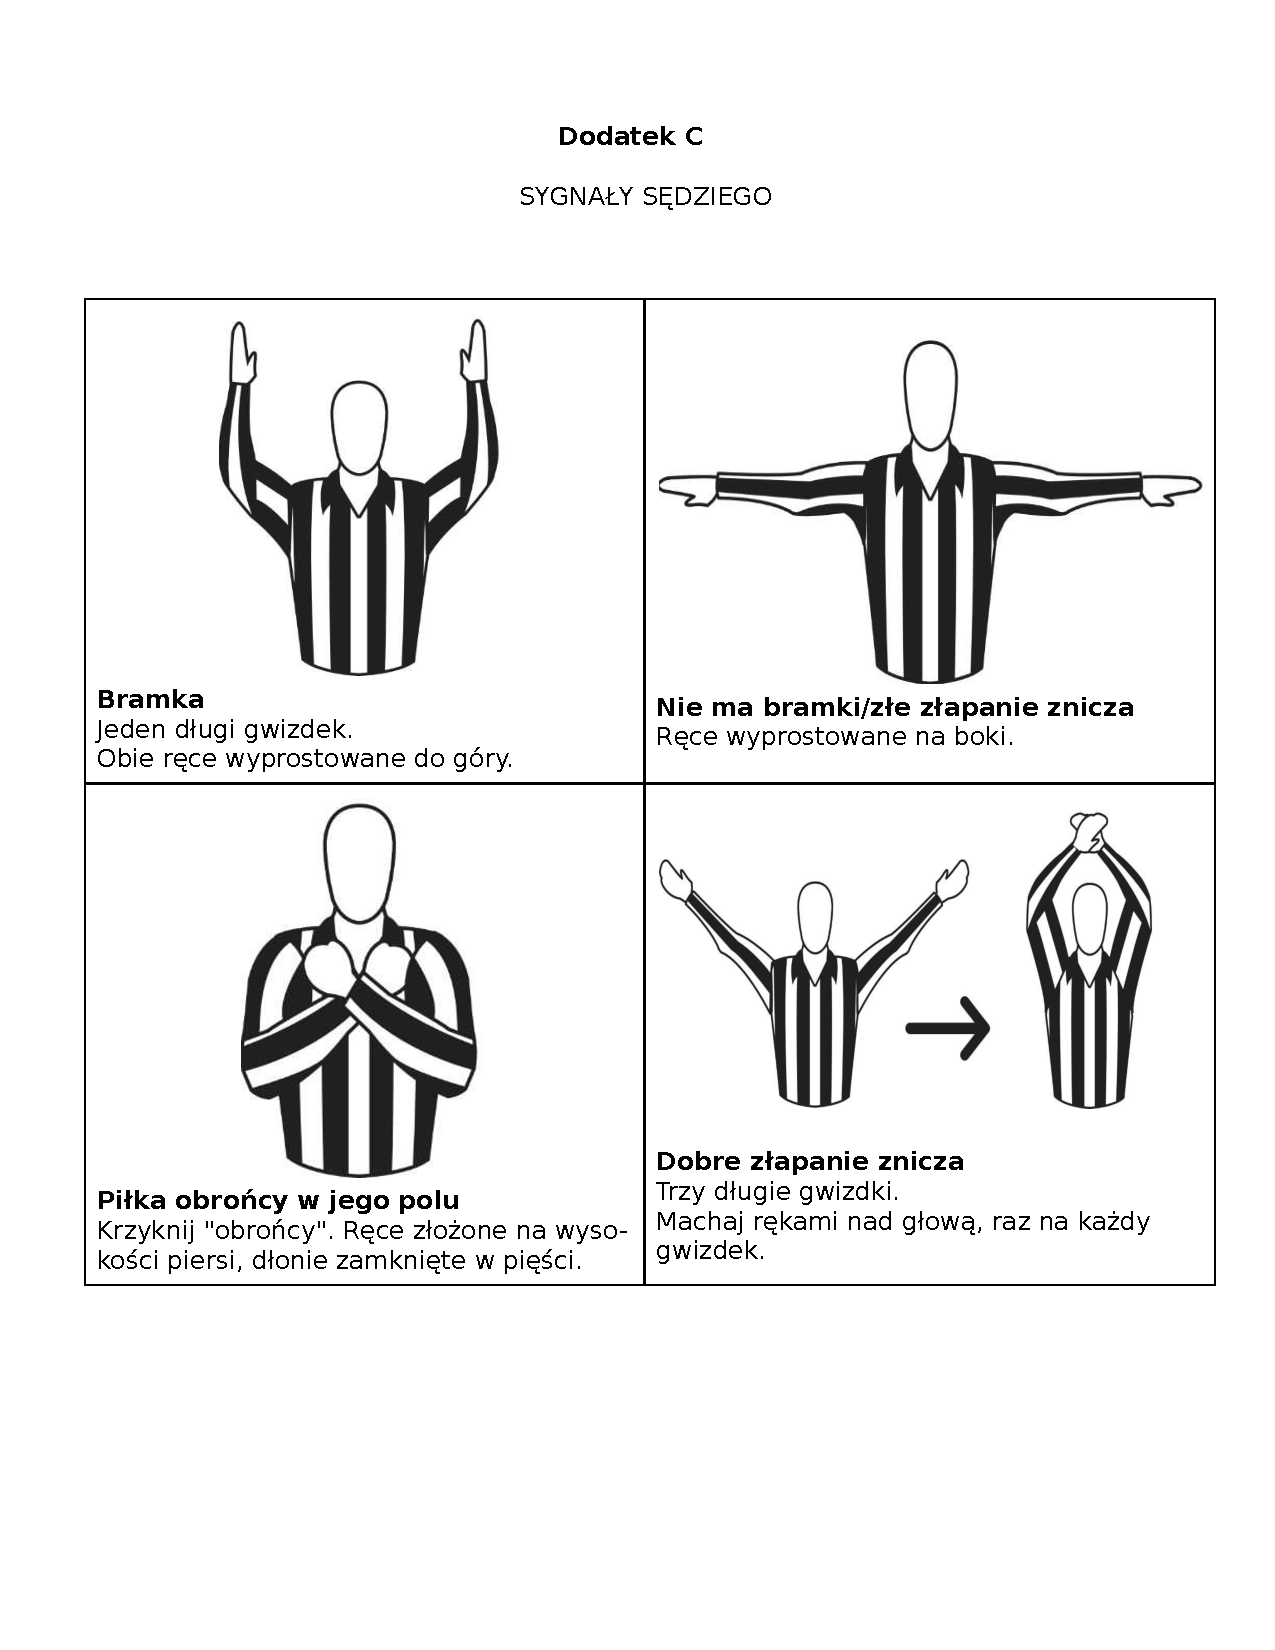
\includepdf[pages={-}]{signals.pdf}

\end{document}
